\documentclass{article}
\usepackage{graphicx}
\usepackage{amsfonts}
\usepackage{tikz}
\usepackage[lined,boxed,commentsnumbered]{algorithm2e}


\begin{document}

\title{CSCI 232 Project: \\ Designing and Implementing a Graph Coloring Algorithm in Java}
\author{Gustavo H. Barrionuevo}

\maketitle

\section{Graph Coloring Problem}

%\section{Graph Coloring}
%\subsection{Basic Definitions}

It is often necessary to partition the vertices of a graph into sets of independent vertices. Suppose that we want to split a group into subgroups which contain only compatible elements, for example, consider the following graph:
\begin{center}
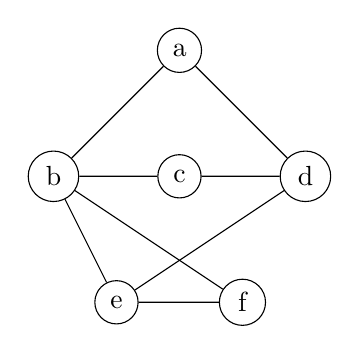
\begin{tikzpicture}
  [scale=.8,auto=left,every node/.style={circle,draw=black,color=black, fill=white}]
  \node (a) at (10,10) {a};
  \node (b) at (8,8)  {b};
  \node (c) at (10,8)  {c};
  \node (d) at (12,8) {d};
  \node (e) at (9,6)  {e};
  \node (f) at (11,6)  {f};

  \foreach \from/\to in {a/b,a/d,b/c,b/e,b/f,c/d,d/e,e/f}
    \draw (\from) -- (\to);

\end{tikzpicture}
\end{center}
A possible partition of independent sets of vertices is: $\{ a \}$, $\{ b, d \}$, $ \{ c, f \}$,$ \{ e \}$. It is clear that is not the best solution. An optimal solution would be: $\{ a, c, e \} $, $ \{ b, d \}$, $ \{  f \}$. In Graph Theory, this problem is showed as a \emph{Graph Coloring Problem} (GCP)\cite{chartrand2008chromatic}.



The formal definition for the GCP is: given a undirected graph $G = (V, E)$, with a set of vertices $V$ and a set of edges $E$, which are incident to the vertices of $G$, the problem is to assign $k$ colors for each vertice in $G$, so that no two adjacent vertices have the same color. So, the \emph{coloring} can be considered as a function $c : V(G) \to \mathbb{N}$ (where $\mathbb{N}$ is the set of positive integers) such that $c(u) \neq c(v)$ where $u$ and $v$ are adjacent in $G$\cite{chartrand2008chromatic}. If $k$ is the minimum number of colors necessary to color the graph, we say that $k$ is the chromatic number of $G$, and it is denoted by $\chi(G)$. Therefore, a graph is $k$-colorable if and only if $\chi(G) \leq k$.  


The GCP can be formulated in two ways. First as a decision problem, where the goal is to identify whether a graph is $k$-colorable. In the second formulation the goal is to find a value $k$ to be minimal.


The study of the GCP has a great theoretical importance because it is a NP-complete problem\cite{MR519066}. Solving this class of problems considered intractable motivates various research in computing, mathematics and operations research.

From a practical standpoint, the study of the GCP is very important because its structure is widely used to model problems in such diverse areas as: scheduling\cite{Lotfi198627}, optimization of register allocation\cite{Chow}, train platforming\cite{Caprara2007129}, frequency assignment\cite{1623376}, communication networks\cite{120165}, and many others.



%\subsection{The Backtracking Algorithm for the k-Coloring Problem}

\section{Analysis and Solution Design}

\subsection{A Backtracking Algorithm for the k-Coloring Problem}

One way to solve GCP would be to generate all possible colorings of the graph. Although this approach will find a solution eventually (if one exists), it is not fast. In this case, for $|V|$ vertices and $k$ colors, there are $k^{|V|}$ different coloring, which means that this brute-force method is feasible just for small numbers of vertices. However, if while generation the possible colorings of the graph we can often avoid  having to check all these colorings. This is exactly what a backtracking algorithm does. 


Backtracking is a modified depth-first search of a tree.  A path from the root to a leaf is a candidate solution. This tree is called a \emph{state space tree}. To determine the solutions, we check each candidate solution in sequence. But it does not take advantage of any signs along the way. We can make the search more efficient by looking for such signs. For example, no two adjacent vertices are the same color. This sign tells us that this node can lead to nothing but dead ends. So, after determining that a node can lead to nothing but dead ends, we go back (``backtrack'') to the node's parent and proceed with the search on the next child. This procedure is caller \emph{pruning} the state space tree.  We call a node \emph{nonpromising} if when visiting the node we determine that  it cannot possibly lead to a solution. Otherwise, we call it \emph{promising}.  
A backtracking algorithm to solve the instance of the GCP is as follows: 
\begin{algorithm}[H]
\DontPrintSemicolon % Some LaTeX compilers require you to use \dontprintsemicolon instead 
\KwIn{$G=(V,E)$ (an undirected graph). Let $S = $ set of vertices that have already been colored together with their color. $S$ is initially empty.}
\KwOut{An assignment of one of $k$ colors to each vertex of $G$}
%$S \gets \emptyset$\;
\eIf{$S = V$} {
    return S\;
} {
 	pick a vertex $v$ not in S\;
 
\For{$C \gets 1$ \textbf{to} $k$}{
	 // verify if some neighbor of $v$ is colored with color $C$ \;
		\If{promising($v$)}	{ 
    add $v$ to S with color $C$\;
    $k\_coloring(G,S)$\;
	}
		}
}
\caption{{\texttt{k\_coloring}:} a backtracking solution to the graph coloring problem.}
\label{algo:coloring}
\end{algorithm}



%Backtracking is used to solve problems in which a sequence of objects  is chosen from a specified set so the the sequence satisfies some criterion. 

%This approach is called $backtraking$ because we are allowed to undo some decisions to go back to a point where a choice was made, then make a different choice and proceed again.


%The algorithm for coloring a graph is somewhat like a search. 

%The space of all possible colorings of the graph - which is considerable larger. For $n$ vertices and $k$ colors, there are $nˆk$ different coloring. we can avoid having to check all these colorings. 

%\begin{itemize}
%\item color all node as being uncolored
%\item go to the first node;
%\item assign a color, and 
%\item go to the next node, and repeat the process
%\item eventually we will either discovery a valid complete coloring or an invalid coloring
%\item if invalid, back up to an earlier node where there are still some choices left and make a different choice, and proceed forward as before.
%\end{itemize}

%Next we present the \emph{promising function} for M-COLORING:

%\begin{algorithm}[H]
%\DontPrintSemicolon % Some LaTeX compilers require you to use \dontprintsemicolon instead 
%\eIf{ neighbor of $v$ is colored with color $C$} {
%    return true\;
%} {
% 	return false\;
% }
%\caption{{\sc promising:} }
%\label{algo:promising}
%\end{algorithm}




 



\subsection{Complexity}



%The GCP is one of a set of very famous problems called $\mathcal{NP}$-complete problems whose known solutions are intractable (the number of cases to test grows exponentially with the input), but for which there is as yet no proof that it must take that much time.

%For a rough analysis of backtracking algorithm.  
%The worst case of backtracking algorithm occurs when no solution exists solely because of a

%The number of nodes in the state space tree for this algorithm is equal to 

For a rough analysis of \texttt{k\_coloring}, consider a less efficient version that does not perform pruning and instead checks the validity of a coloring only when a coloring
is complete. In the worst case, the algorithm must check the validity of every possible node in the state space tree, which is equal to:
\begin{equation}
1 + k + k^2 + \dots + k^{|V|} = \frac{k^{|V|+1}-1}{k-1}
\end{equation}
Thus the running time for this algorithm is bounded above by $O(k^{|V|})$. 

Although backtracking algorithms for problems such as the GCP are still exponential-time in the worst case, they are useful because they can be efficient for a particular large instance.

%Although backtracking algorithms for problems such as the GCP are still exponential-time in the wort case, they are useful because they are efficient for many large instances, not because they are efficient for all large instances. 


%Although this approach will find a solution eventually, it isn't speedy. Backtracking over $n$ variables, each of which can take on $k$ possible values, is $O(k^n)$.


%In the worst case, the algorithm must check the validity of every possible complete coloring. Since there are $k$ ways to color each vertex and $|V|$ vertices, there are $kˆ{|V|}$ complete colorings of the graph. For each complete coloring, the validation check must examine the pair of adjacent vertices corresponding to each edge. 



%complete coloring. Since there are $k$ ways to color each vertex and $n$ vertices, there are $kˆn$ complete colorings of the graph. For each complete coloring, the validation check must examine the pair of adjacent vertices corresponding to each edge. 

%Although this approach will find a solution eventually (if one exists), it isn't speedy. Backtracking over n variables, each of which can take on k possible values, is $O(k^n)$.


\section{Algorithm Behaviour: Experimental Analysis}




\subsection{Experiment Setup and Procedure}

Among the possibilities of instances that could be used to analyze the performance of the algorithms, the following types of graphs were chosen and listed below, based on 10 runs in each set, totaling 900 different instances of graphs.



\begin{itemize}

\item DENSE:  30 randomly generated graphs of which the number of vertices varies uniformly in the range $ n \in [ 100 , 3000 ] $ with a probability of connection between vertices defined in $70\%$ . These graphs are part of the set of instances testing for presenting a high value for $\chi(G)$, and therefore are the ones that require more computational time to be colored. In this scenario we analyzed 300 graphs.
	
\item LARGE: 30 randomly generated graphs of which the number of vertices is fixed at $n = 1000$ and its density varies uniformly between $1\%$ and $99\%$. With this set of instances, we intend to analyze the influence of $\chi(G)$ variation on the computational time of the studied algorithm. In this scenario , we analyzed 300 graphs.
	
\item REGULAR: 30 graphs $k$-regular randomly generated  with the fixed number of vertices in $n = 1000$ and the value of $k$ varying uniformly between 30 and 999. With this set of instances, it is intended to determine whether the high symmetry in this graph $k$-regular can influence the computational time. In this scenario, we analyzed 300 graphs.

\end{itemize}

It is believed that the selected instances covers all the important features to be studied in this text. Other types of graphs such as  planar or  bipartite graphs were not considered. 

\subsection{Data Analysis}

In all the graphs to be displayed, each point on the graph represents the average of 10 runs of the algorithm studied. 


% The graph of Figure~\ref{fig:dense} shows the average of 10 runs of staining results of ratio values ​​found for the dense graphs

\begin{figure}[!htb]
\label{fig:dense}
{\centering 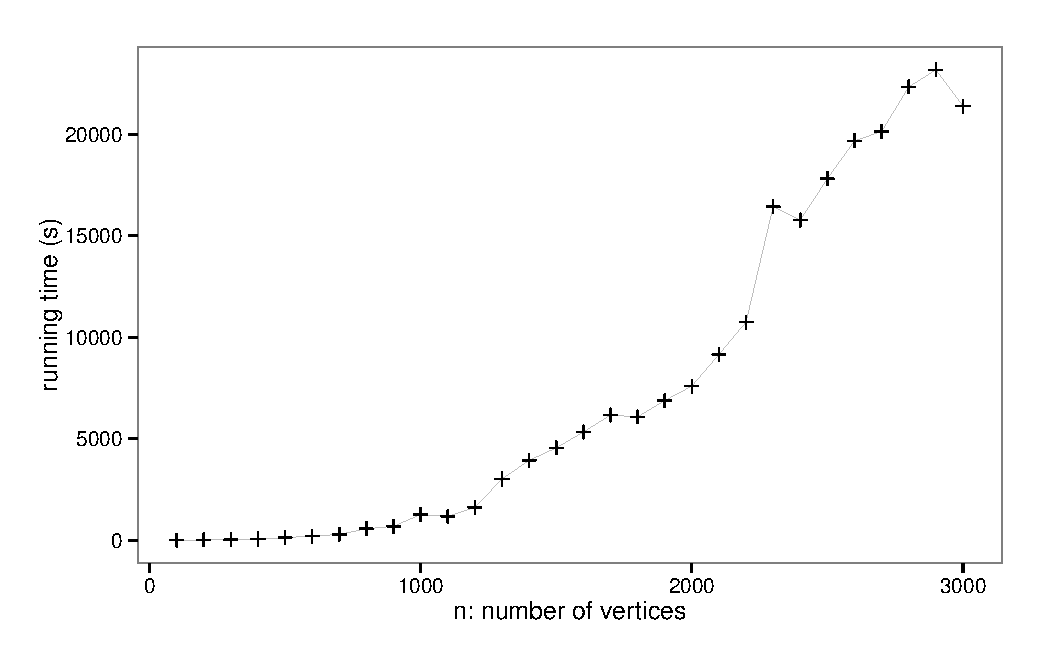
\includegraphics[width=1\textwidth]{dense} 
\caption{Running time of dense graphs with probability of connectedness $p=0.70$.}
}
\end{figure}



%In the graphs of Figures~\ref{fig:large} and~\ref{fig:regular} we can see that the same behavior also appears to set LARGE and REGULAR .


\begin{figure}[!htb]
\label{fig:large}
{\centering 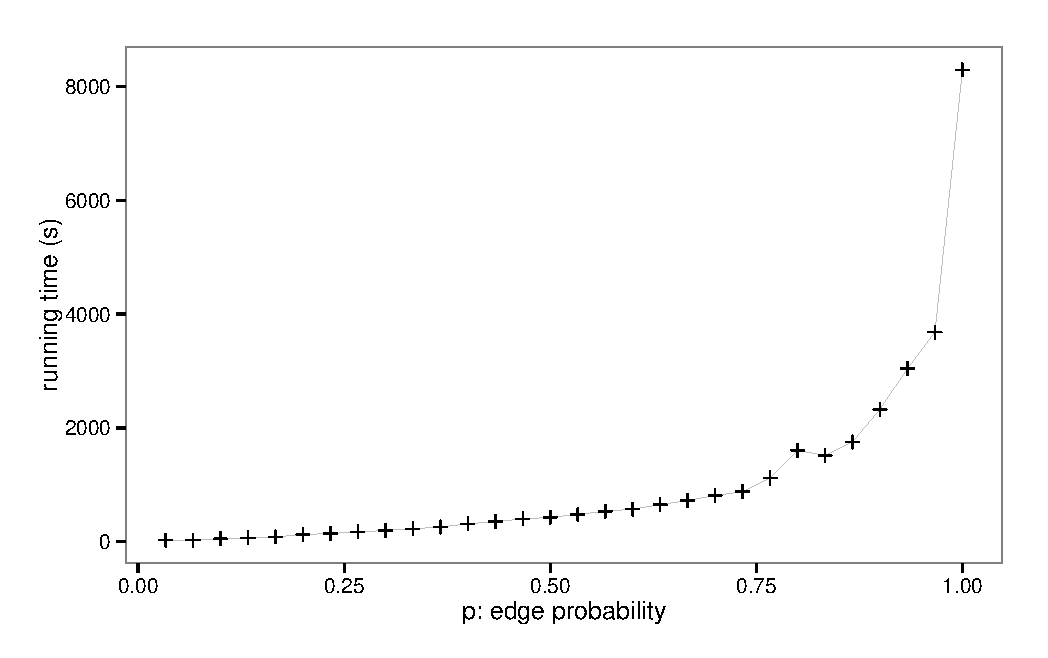
\includegraphics[width=1\textwidth]{large} 
\caption{Running time of large graphs with 1000 vertices.}
}
\end{figure}


\begin{figure}[!htb]
\label{fig:regular}
{\centering 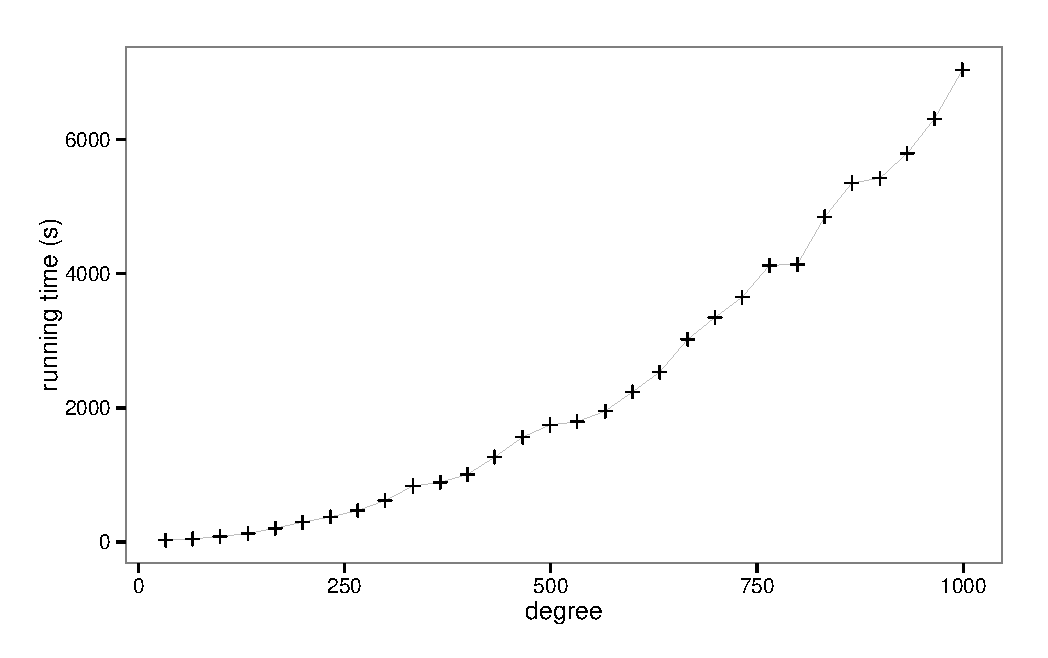
\includegraphics[width=1\textwidth]{regular} 
\caption{Running time of regular graphs with 1000 vertices.}
}
\end{figure}

%The empirical results confirm the bounds on the running time and the solution quality as claimed in the theoretical paper. 

%Considering the results presented, 

%instances testing for presenting a high value for $\chi(G)$, and therefore are the ones that require more computational time to be colored. it's not possible to conclude each one if there is a specific t


% The results show that for theses three type of graphs (DENSE, LARGE, REGULAR) have a exponential grow.  the behavior 


% the algorithm is likely to perform much better than the theoretical analyses suggests. But the results suggest that the algorithm might be well suited for edge coloring graphs quickly and efficiently in graphs with a low chromatic number and large number of vertices.



%Considerando os resultados apresentados, não podemos dizer qual dos três tipos de grafos o algoritmo apresenta melhor desempenho. Mas podemos observar aqui que o 
%\section{Discussion}

%\section{Conclusions}


\bibliographystyle{ieeetr}
\bibliography{refs}

\end{document}

